%!TEX root = ../tese.tex
%!TEX encoding = UTF-8 Unicode
\chapter{Implementation}\label{chapter:implementation}
This chapter addresses the main decisions adopted regarding the implementation of the intrusion recovery system Shuttle. Shuttle is supposed to be implemented by the \ac{PaaS} providers since it requires modifications to the \ac{PaaS} system and database service.

%button-up approach. What are the base technologies?
\section{Adopted Technologies}\label{sec:impl:adopted_technologies}
%Criteria
In order to implement the proposed work, we evaluated several technologies taking in account the requirements of the problem and the performance, scalability and easiness of implementation in a production mode \ac{PaaS} provider service.
%Python
The first Shuttle prototype was implemented in Python. The prototype of a simple application and the proxy allowed to analyze the requirements of Shuttle. The compact code of Python was great for code readability and rapid prototyping. However, despite the stackless variants of Python, the global interpreter lock limits Python to a single active thread per process. Since all modules of Shuttle are multi-threaded and their performance is critical to support medium and large-scale systems, Python was not appropriated. The selected language needs to be likely to run faster than Python and to have better concurrency and network libraries.

%C and C++
C or C++ languages are likely to have a better performance than Python because they are compiled. However, the development time can be considerably larger due to its low level. 
Java has a higher abstraction level than C but lower than Python. To argue about the performance differences between Java and Python, we would need to develop a version of Shuttle in Python and another version in Java. However, the proxy prototype using Java has a bigger throughput and lower latency than the one implemented using Python. 

%Scala, Go, Erlang
Shuttle has a distributed architecture and each module shall process various requests concurrently. Therefore, we also considered languages, such as \emph{Erlang}, \emph{Go Lang} and \emph{Scala}. They facilitate the writing of concurrent programs that share the state by communicating. Moreover, the actors model \cite{actors}, native in Erland and available through frameworks as Akka \cite{akka} to Scala, could simplify the implementation and improve the performance. 

%Java
Java is still the most used language in enterprise environments and it is compatible with most of \ac{PaaS}. The selected database is implemented in Java (Chapter \ref{sec:impl:database_options}). In addition, Java has the \ac{NIO} library that provides event-driven and asynchronous communication via network. %Due to its broad usage, Java is more likely to have client libraries for distributed databases than other languages, for instance C.

%Why not Java?
We chose to implement the Shuttle prototype in Java. However, the large number of concurrent tasks and asynchronous message passing communications turned the development of the prototype using Java extremely complex. Moreover, its concurrency model and network libraries have an abstraction level lower than desired to archive a fast development and good performance.

Therefore, during the development of the prototype, we concluded that \emph{Scala} with \emph{Akka} could be a better option than Java. It would be likely to simplify the development of the distributed system and improve the performance. However, rebuilding the prototype in a different language would also take too long. Therefore, we kept Java.
In addition, the proxy performance could be improved using a C or C++ implementation, such as HAProxy \cite{haproxy}. \\

Shuttle is built of several modules that communicate and coordinate their actions. We choose to use a messaging protocol instead of \ac{RPC} (such as Java \ac{RMI}). The message passing protocol should emphasized simplicity, performance and low overhead. It should also define data structures and service interface easily. 

Plain text protocols are communication protocol whose content representation is intended to be read by humans. For instance, the \ac{SOAP} \cite{soap} specifies rules for using XML to package messages. Despite the heterogeneity and easiness of debug of plain text protocols, the text encoding and message structure has a significant overhead. As opposed, binary protocols are intended to be read by machines. The advantage of compactness translates into smaller messages and faster transmission and interpretation than plain text protocols. The capability of describe data structures using an \ac{IDL} and generate the source code in various programming languages to generate and parse the stream of bytes is also important to reduce the period of implementation and support transparent interaction between multiple programming languages. To cope with these requirements, we selected a binary protocol with \ac{IDL}. 

Apache Thrift \cite{Thrift} and Google's Protocol Buffer \cite{protobuffers} are two of the current binary communication protocol that fit these requirements. These protocols are similar, the main difference is the first offers a stack implementation for \ac{RPC} calls. The exact performance differences between them can only be measured benchmarking the two possible implementations. We choose Protocol Buffers to implement our prototype.



%%%%%%%%%%%%%%%%%%%%%%%%%%%%%%%%%%%%%%%%%%%%%%%%%%%%%%%%%%%%%%%%%%%%%%%%%%%%%%%%%%%%%%%%%%%%%%%%%%%%%%%%%%%%%%%%%%%%%%%%%%%%%
\subsection{Platform as a Service}\label{sec:impl:paas}
Shuttle is implemented as a service in \ac{PaaS} framework. Since we can not modify the implementation of \ac{CSP} solutions, such as Google App Engine \cite{GoogleAppEngine} and Amazon Web Services \cite{AmazonElasticBeanstalk}, we chose an open-source \ac{PaaS} framework. The framework has to meet the following requirements: 

\begin{enumerate}
	\item \textit{Open-source:} to support updates and modifications
	\item \textit{Support to add new containers:} to add new compute, database and replay instances.
	\item \textit{Contain a load-balancer:} to distribute the requests after the proxy
	\item Extensible to support a new database management system
	\item Deployable on OpenStack and \ac{AWS}
	\item Support for Java Applications
\end{enumerate}

We consider the auto-scaling capability as optional since Shuttle may invoke the \ac{PaaS} manager to create new application instances, database instances and replay instances. However, the capability to monitoring the containers usage during the recovery period turns the replay process faster and cost-efficient by adjusting dynamically the required resources (Chapter \ref{sec:eval:peformance}). 

We require the \ac{PaaS} system to be deployable on OpenStack \cite{openstack} and \ac{AWS}. Due to the costs of a public cloud service, the prototype is tested in a local cloud supported by OpenStack and later on a public cloud \ac{AWS}.


We chose AppScale \cite{Appscale} to implement our prototype. AppScale meets the requirements except it does not support OpenStack nether supports the required database (Chapter \ref{sec:impl:database_options}).  Therefore, we contributed for AppScale open-source project adding the support for both. AppScale supports auto-scaling monitoring the proxy and nodes: if one of the servers queue contains more than 5 requests or if the node usage exceeds the 90\%, then it creates a new container and deploys the application. There are many alternatives being actively developed. The main open-source systems are Openshift by RedHat \cite{OpenShift}, AppScale \cite{Appscale}, Apache Stratos \cite{ApacheStratos}, Cloud Foundry \cite{Cloudfoundry}, Cloudify \cite{cloudify} and Solum project of OpenStack \cite{solum}.  


\subsection{Database}\label{sec:impl:database_options}
%Database normal:	
Shuttle could be implemented in \ac{PaaS} supported by most of known databases, including relational (\ac{SQL}) databases (Database instances in Figure \ref{fig:shuttle_architecture}). However, previous projects encompass relational databases \cite{warp,goel} and \ac{PaaS} applications are often supported by \acs{NoSQL} databases. Shuttle is the first intrusion recovery system using replay considering \acs{NoSQL} databases.

%why nosql
\acs{NoSQL} databases are designed for extremely large data sets, hundreds or thousands of million entries. Most of the architectures of \acs{NoSQL} databases claim to scale horizontally near linearly, i.e., adding twice the data means to add twice the nodes. To do so, the data of \acs{NoSQL} storages is partitioned across multiple servers, for instance, by a range of keys or using consistent hashing \cite{Chang2008}. Therefore, \acs{NoSQL} stores can compensate the overhead imposed by Shuttle distributing the data across the nodes, scaling horizontally instead of vertically. 


Unlike relational databases, \acs{NoSQL} databases do not guarantee \ac{ACID} properties. One of the main differences between the \acs{NoSQL} storages is their approach to preserve consistency or availability during the network partitions. The \acs{CAP} theorem states any networked shared-data system can have at most two of the three desirable properties: consistency, availability and tolerance to network partitions \cite{brewer2012cap}.

\acs{NoSQL} databases support new data structures, which are more flexible than the schema of relational databases:
 \begin{enumerate}
 	\item \textit{Column-oriented:} The data is organized in a multidimensional persistent sorted map with a large number of key-value pairs within rows.
  	\item \textit{Document-oriented:} The format of the values is a JSON or JSON like document. Documents are organized in collections. The document attributes can be included in the query.
  	\item \textit{Key-value:} Similar to a map where the values are opaque and accessed by an unique key.
  	\item \textit{Graph:} Heavily linked data with multiple relations.
  \end{enumerate} 

The evaluated alternatives are summarized in Table \ref{tab:no_sql_databases}. 




\begin{center}
\rowcolors{0}{}{lightgray}
\begin{table}[ht]
\begin{tabular}{|m{1.5cm}|m{1.8cm}|m{1.6cm}|m{1.8cm}|m{1.7cm}|m{5cm}|}\hline
\textbf{Type}  & \textbf{Name} & \textbf{Language} & \textbf{API} & \textbf{Replication}  & \textbf{Consistency} \\ \hline

\multirow{2}{*}{Column} 
	& HBase 		& Java  & Avro, REST, Thrift & Master-Slave & Strongly consistent for a single row within a datacenter. Across rows is eventual consistent \\ \cline{2-6}
	& Cassandra 	& Java  & Cassandra Query \newline Language & Peer-to-peer  & Depends on the selected number of read and writes \\ \hline

\multirow{2}{1.5cm}{Document Oriented} 
	& MongoDB  	& C++  		& \acs{CRUD}  	& Master-slave & Strong Consistency for a single row (default) \\ \cline{2-6} 
	& CouchDB 	& Erlang   	& \acs{CRUD} 	& Master-slave & Multi-Version Concurrency Control \\ \hline

Graph 
	& Neo4J 	& Java  	& Cypher Query \newline Language  & Master-Slave & ACID using master. Updates to slaves are eventual consistent by default \\ \hline


\multirow{2}{1.5cm}{Key value}         
	& Memcached   	& C  		& \acs{CRUD}  	& None 			& The client selects the correct shard \\ \cline{2-6} 
	& Voldemort  	& Java		& \acs{CRUD} 	& Peer-to-peer 		& Many-writer eventually consistent system: vector clocks and versioning  \\ \hline
\end{tabular}
\caption{Available No \ac{SQL} databases}
\label{tab:no_sql_databases}
\end{table}
\end{center}

HBase and Cassandra follow the Google Big Table column-oriented database \cite{Chang2008}. HBase has master-slave architecture and provides get, put, delete operations but also scan, server-side atomic operations and atomicity on row-level writes. Cassandra has a peer-to-peer architecture based on Dynamo \cite{Decandia2007}. The consistency of the operations is determined per-operation basis by the number of read and written replicas. Strong consistency requires to read/write a quorum while on eventual consistency the storage system guarantees that if no new updates are made to the object, eventually all accesses will return the last updated value. \cite{Decandia2007}. Cassandra resolves conflicts using the timestamp and a last-write-wins policy. 

MongoDB and CouchDB are two of document-oriented stores. Their \ac{API} allows to \ac{CRUD} documents. MongoDB has master-slave architecture: one master per shard (a partition of the key-space) and the shard's slaves are eventual-consistent. Therefore, there are no conflicts. On other hand, CouchDB records any changes as a version of the document and allows conflict resolution via programmatic merge. 

Graph stores such as Neo4J target a specific kind of applications.

Memcached and VoldemortDB are in-memory distributed key-value stores. Memcached does not provide a replication mechanism by default and it is often used to cache web pages. Like CouchDB, VoldemortDB is an eventual consistent store that accepts asynchronous concurrent writes.\\

The correct \acs{NoSQL} database depends on the particular application, which has different size of data sets, complexity, rate between writes and reads, consistency requirements and methods to access the data. Column-oriented is beneficial for applications that must access a subset of values. Key-value structure is beneficial for applications that retrieve entire values. 

We selected VoldemortDB \cite{Kreps} to implement Shuttle. Voldemort is an open source implementation of Dynamo \cite{Decandia2007}, which is the base of DynamoDB provided on \ac{AWS}. Voldemort is a key-value store developed and in used by Linkedin \cite{linkedin}. Voldemort has a put, get, delete, update (\ac{CRUD}) \ac{API} so we avoid the delay of parsing complex queries. Voldemort does not allow range queries, i.e., the user can retrieve only one value each time, so data items accessed by them are known before the request execution and, consequently, we expect fewer false dependencies (Section \ref{sec:arch:dependencies}). 


Voldemort accepts asynchronous concurrent writes and treats the result of each modification as a new and immutable version of the data. Versions of the data can conflict if two or more replicas are updated concurrently during a network partition. A network partition occurs when a failure causes the system to be partitioned in multiple sub-systems and two nodes of the system cannot communicate. When the network partition is healed, Voldemort uses the vector clock of each version to determine the causality between those versions \cite{Decandia2007}. A conflict exists if two versions do not have a causality relation. Voldemort resolves the conflicts during the following read operation. The conflict is solved is application-assisted: the application reads both versions and based on its semantics, the application chooses the correct version. We leverage the semantic reconciliation to solve distinct parallel replay with different execution (Section \ref{sec:arch:dependencies}).

Voldemort keeps the persistent state on a local transactional database: BerkeleyDB, MySQL or an in-memory key/value data structure. It also allows to choose the serialization protocol, for instance: Java Serialization, Avro, Thrift and Protocol Buffers, which is also used by Shuttle as message passing protocol. Since Voldemort is open-sourced therefore we can modify its implementation to include the Shuttle requirements. We used the release 1.9.0 of Voldemort backed by BerkeleyDB and serialized using Protocol Buffers.

On an earlier stage, we considered and attempted to implement Shuttle on MongoDB. However, MongoDB is implemented using C++, does not support conflict solving and it extends the \ac{CRUD} \ac{API} with further complex operations such as scans. A future work may concern the implementation on a column-oriented database, such as Cassandra.\\

The \emph{Shuttle Storage} stores for each request: the \ac{HTTP} request, \ac{HTTP} response, the accessed keys and the start and end instants. Since an application is expected to retrieve hundreds or thousands of million requests, the data set stored in Shuttle Storage is expected to be extremely large. The size of each data item is expected to be on dozens of kilobytes. The write operations are frequent while the read operations occur during the recovery process. Each data item is written twice: once to add the request, response and start/end timestamps and once to add the accessed keys. The storage must be available during the recovery process and may be replicated to a remote site to prevent catastrophic disasters. Conflicts may occur within a data item: one version containing the request/response, the other containing the accessed keys. Therefore, eventual consistency is tolerated if the database management system is able to solve conflicts within the data item. At last, the fields of each data item are known and immutable.

Taking into account the above requirements, we selected to implement the prototype using Cassandra \cite{Lakshman2010a} as Shuttle storage. Cassandra keeps the versions per-column so it can resolve conflicts within the data item. In addition, it allows to choose the number of read and write servers. Due to the simple content format and the required operations, most of distributed databases, including Amazon's DynamoDB, Google's Cloud Datastore, fulfill the defined requirements.

The external storage should be protected, at least, against attacks to integrity and confidentiality. If the integrity of at least one request is affected, then Shuttle can not replay the requests previous to the most recent affected request and the application is unrecoverable if a snapshot following that period does not exists. For sake of simplicity, we ignore the security features of the Shuttle storage in this implementation as we consider the Shuttle storage to be part of the trusted computing base.








%%%%%%%%%%%%%%%%%%%%%%%%%%%%%%%%%%%%%%%%%%%%%%%%%%%%%%%%%%%%%%%%%%%%%%%%%%%%%%%%%%%%%%%%%%%%%%%%%%%%%%%%%%%%%%%%%%%%%%%%%%%%%
\section{Normal Execution}\label{sec:impl:normal}

Shuttle can operate in one of two states: \textit{normal execution} and \textit{recovery}. During normal execution, Shuttle collects  dependencies between requests, stores the accessed data items, sets the correct branch to write the data item values and performs snapshots. Figure \ref{fig:normal:mensaging} summarizes the messages exchanged between Shuttle's modules during the normal phase. Shuttle identifies each user \ac{HTTP} request with an unique \ac{SRD} and identifies all database operations of each request with its \ac{SRD}. The database operations are logged and sent to the manager, which generates the dependency graph. 
In this Section, we describe the normal execution phase following the path that a request takes to be processed.

\begin{figure}
  \centering
  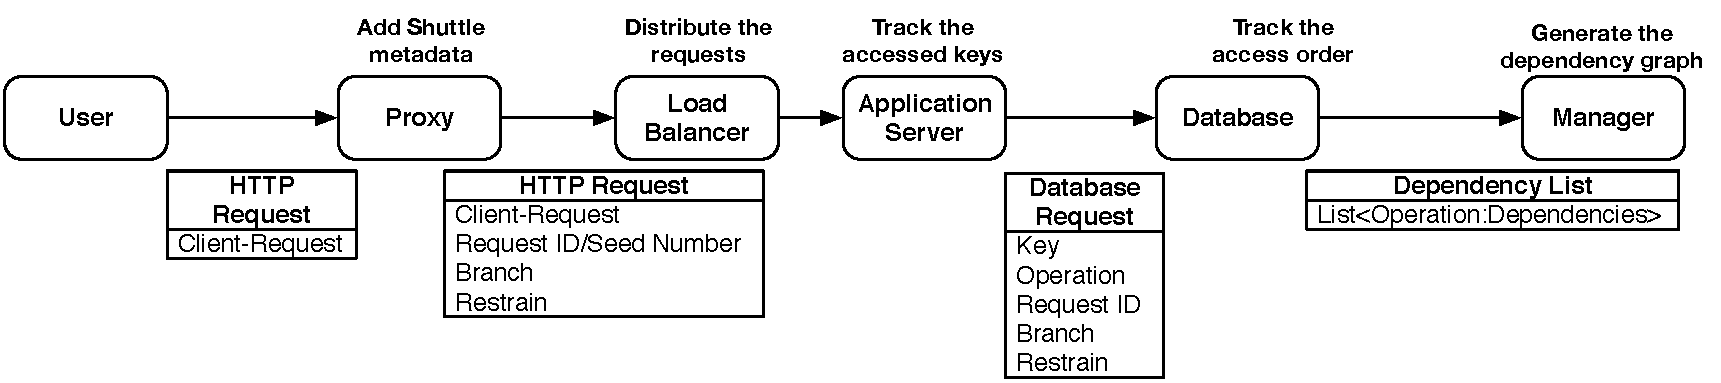
\includegraphics[width=\textwidth]{images/message_normal}
  \caption{Interactions between components during normal execution}
  \label{fig:normal:mensaging}
\end{figure}



%%%%%%%%%%%%%%%%%%%%%%%%%%%%%%%%%%%%%%%%%%%%%%%%%%%%%%%%%%%%%%%%%%%%%%%%%%%%%%%%%%%%%%%%%%%%%%%%%%%%%%%%%%%%%%%%%%%%%%%%%%%%%
\subsection{Proxy}\label{sec:impl:normal:proxy}
The proxy retrieves all \ac{HTTP} user requests and adds the \ac{SRD} to their headers. The \ac{SRD} contains the following fields:
\begin{enumerate}
	\item \ac{RID} (long).
	\item Branch: the branch accessed by the request (short).
	\item Restraint: to support branch change during the recovery phase (boolean).
\end{enumerate}

The proxy could be implemented by modifying an existing open-source proxy, e.g., HAProxy or Nginx. They are well tested in production and implemented in C. Moreover, they are likely to perform better than a prototype using a higher-level language, such as Java (Section \ref{sec:eval:performance:proxy}). However, for sake of expected simplicity, we implemented a new \ac{HTTP} proxy using Java. Nevertheless, implementing most part of the \ac{HTTP} protocol specification in an efficient manner using Java ended up to be a complex task.


\begin{figure}
  \centering
  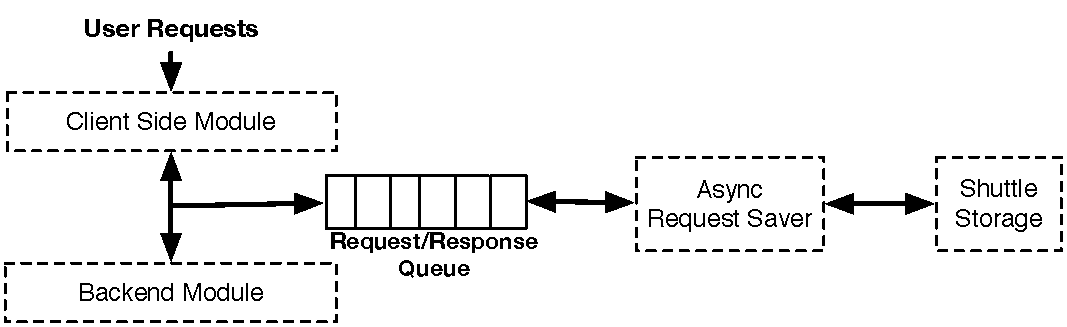
\includegraphics[width=0.7\textwidth]{arch/proxy}
  \caption{Proxy internal modules}
  \label{fig:impl:proxy_modules}
\end{figure}

The proxy is made of three parts: the client-side module, the backend module and the asynchronous request saver (Figure \ref{fig:impl:proxy_modules}).

The client side module retrieves \ac{HTTP} requests, parses their content and modifies their headers. We used the \ac{NIO} library of Java to implement a TCP server. The server retrieves user requests and modifies their header (Algorithm \ref{code:proxy_service}). The values of \emph{branch} and \emph{restrain} are defined by the Shuttle's manager while the \ac{RID} is a timestamp of the proxy instance. Java provides timestamps with a precision of millisecond. This precision limits the proxy performance to one thousand requests per second. Therefore, we used a counter to identify the same millisecond, up to 1000 requests per millisecond (1 million requests per second). The precision of the timestamp weights on the network and storage overhead. The \ac{RID} is also used as a timestamp for the application and as a pseudorandom number generator, so the request generates always the same sequence of non-repeating numbers. The fields of \ac{SRD} represent a fixed overhead of 35 ASCII characters, corresponding to 35 bytes, in every request header.

Proxy's TCP client threads send the requests to the load balancer. We use a fixed size thread pool to associate each \ac{HTTP} response to the correct \ac{HTTP} request. The thread that retrieves, processes and forwards the request to the load balancer, blocks until its response is retrieved. When the response is retrieved, the Proxy associates a \emph{end-timestamp}. A future work shall implement the proxy as a fully asynchronous proxy. To do so, the application server shall include the \ac{SRD} in the responses. Since the delay of creating a new TCP connection to the load balancer is considerable, our implementation keeps the TCP session with the load balancer and implements the \ac{HTTP} keep-alive specification. \ac{HTTP} keep-alive is a standard that allows a single TCP connection to send and receive multiple \ac{HTTP} requests/responses, instead of opening a new connection for every request/response pair. 

\begin{algorithm}
	\DontPrintSemicolon\SetKwProg{fn}{Function}{}{}
		\KwIn{received user \ac{HTTP} request}
		\KwResult{user \ac{HTTP} request with modified header}
		\SetKw{KwInit}{Initialization:}\KwInit{establish a \ac{HTTP} connection to the load-balancer}\;
		\BlankLine 
		\Letv{package}{Read TCP package from client}\;
		\Letv{request}{Parse $package$ to bound \ac{HTTP} request}\;
		\Letv{SRD}{Get Shuttle's state: $id, branch, restrain$}\; 
		Add $SRD$ fields to request's header formated as: \newline ID: $id$ \newline B: $branch$ \newline R: $restrain$\;
		Send $request$ to load balancer\;
		Add $SRD$ and $request$ to $queue$\;
		\tcc{Retrieve response}
		\Letv{package} {Read TCP package from load balancer}\;
		\Letv{response} {Parse $package$ to bound \ac{HTTP} response}\;
		\Letv{endTimestamp} {get current system time}\;
		Send $response$ to client\;
		Add $endTimestamp$ and $response$ to $queue$\;
  	\caption{Proxy}
	\label{code:proxy_service}
\end{algorithm}



%how to store the data?
Shuttle proxy stores $requests$, $responses$, $end-timestamp$ and $SRD$ in the Shuttle storage. If the data would be sent synchronously to the storage, then the response delay would increase. Therefore, we implemented a message queue (Figure \ref{fig:impl:proxy_modules}). The client-side and backend module add the data as a message in the queue. Worker threads dequeue the messages and store the data in Cassandra. This allows asynchronous behavior: requests can proceed before the transmission has finished. The worker threads are wake when the queue reaches a defined threshold or a timeout period expires. The message queue is implemented as a \emph{synchronized list} in Java.


 %%%%%%%%%%%%%%%%%%%%%%%%%%%%%%%%%%%%%%%%%%%%%%%%%%%%%%%%%%%%%%%%%%%%%%%%%%%%%%%%%%%%%%%%%%%%%%%%%%%%%%%%%%%%%%%%%%%%%%%%%%%%%
\subsection{Application Server}\label{sec:impl:normal:compute}
%Goals
The Shuttle implementation in application servers shall meet two architecture requirements: log the database accesses per request and include the requests' \ac{SRD} on every database invocation. We want to limit the number of hooks in the application and avoid modifying the database \ac{API}. The database service \ac{API} shall remain equal so as the tenants' applications code. Shuttle shall be transparent to application developers.\\


%how to pass the ID?
Shuttle architecture establishes that every database operation must include the \ac{SRD}. The first solution would implement directly the architecture in Figure \ref{fig:shuttle_architecture}, in which a proxy that modifies every database request or modify the database client \ac{API} to include the \ac{SRD} as an argument. However, for the sake of simplicity, we modified the Voldemort client to include the \ac{SRD} field on every database operation. We modified the Voldemort messages, which are described using \ac{protobuf} \acs{IDL} (Appendix \ref{appendix:voldemort_api}). The implemented \emph{interceptor} gets the \ac{SRD}, which is written in request header, tracks the access and invokes the modified Voldemort client (Algorithm \ref{code:database_client_interceptor}).

\begin{algorithm}
\DontPrintSemicolon\SetKwProg{fn}{Function}{}{}
\SetKwFunction{Put}{put}\SetKwFunction{VPut}{voldemort.put}\SetKwFunction{AddKey}{trackKeyAccess}
 
 \fn{\Put{key, value, store}}{
  \Letv{srd}{\AddKey(key, store, "put")} \tcp*{get SRD and track access(Algo.\ref{code:interceptor_code_access})}
  \VPut{key, value, srd}\;
  }{}
\caption{Voldemort \ac{API} interceptor (example of put operation)}\label{code:database_client_interceptor}
\end{algorithm}

In order to extract the \ac{SRD} from the requests' header, we took in account that \ac{PaaS} systems deploy applications in application engines. Specifically, AppScale deploys the Java applications on the servlet engine WildFly \cite{wildfly} (formerly known as JBoss). In addition, most of Web Service frameworks, e.g., \ac{JAX-WS}, and \ac{MVC} frameworks, such as Spring, encompass the concept of interceptor chain, also known as filters or handlers. An interceptor chain is a sequence of handlers that contain methods that are invoked before and after the request processing by the application controller.

We implemented a \emph{request interceptor} in Spring. Application developers only need to add a single line to their applications \emph{web.xml} file to add the developed interceptor to the interceptor chain. A future work may concern the implementation interceptor for other application engines.

We also took into account that each request in Spring is binded to a single thread. Therefore, Shuttle keeps an hash table that associates the \ac{TID} with the \ac{SRD} and list of accessed keys of the request that it is processing. The \emph{request interceptor} parses the request header and creates an entry in the hash table (Algorithm \ref{code:interceptor_code_pre}).


\begin{algorithm}
\DontPrintSemicolon\SetKwProg{fn}{Function}{}{}
\SetKwFunction{PreHandle}{preHandle}\SetKwFunction{MapPut}{map.put}
\SetKwFunction{TrackAccess}{entry.trackKeyAccess}

	\KwData{$map$ is a static hash table}
	\KwIn{HTTP user request}
	\BlankLine
	\fn{\PreHandle{request}}{
		\Letv{keySet}{new empty list}\;
		\Letv{srd}{parse request header}\;
		\Letv{tid}{get current thread id}\;
		\Letv{entry}{create entry pair: \{$keySet, srd$\}}\;
		\MapPut{tid, entry}\;
	}{}
	\caption{Shuttle interceptor: Pre handler}
	\label{code:interceptor_code_pre}
\end{algorithm}

Before every database operation, the database client library invokes the client interceptor to log the access. The interceptor resolves the \ac{TID} into the request's \ac{SRD}, adds the new key to the set of accessed keys of the \ac{SRD} and returns the \ac{SRD} (Algorithm \ref{code:interceptor_code_access}). The client library appends the \ac{SRD} in the database operation request. 


\begin{algorithm}
\DontPrintSemicolon\SetKwProg{fn}{Function}{}{}
\SetKwFunction{AddKey}{trackKeyAccess}\SetKwFunction{TrackAccess}{entry.addKeyAccess}
\SetKwFunction{MapGet}{map.get}
	
	\fn{\AddKey{key, store name, operation type}}{
		\Letv{tid}{get current thread id}\;
		\Letv{entry}{\MapGet{tid}}\;
		\TrackAccess{key,store name, operation type}\;
		\Return{$entry.srd$}
	}{}
\caption{Shuttle interceptor}
\label{code:interceptor_code_access}
\end{algorithm}

The post-process interceptor (Algorithm \ref{code:interceptor_code_pos}) accesses the map extracting the accessed keys and the \ac{SRD} of the current thread. The accessed keys are stored among the \ac{HTTP} request/response in the Shuttle storage. In addition, this interceptor also adds the \ac{SRD} to the response header.

\begin{algorithm}
\DontPrintSemicolon\SetKwProg{fn}{Function}{}{}
\SetKwFunction{AfterCompletion}{afterCompletion}\SetKwFunction{MapRemove}{map.remove}
\SetKwFunction{StorageAdd}{shuttleStorage.add}

	\KwData{$map$ is a static hash table}
	\KwIn{HTTP user request and \ac{HTTP} response}
	\BlankLine
	\fn{\AfterCompletion{request, response}}{
		\Letv{entry}{\MapRemove{tid}}\;
		\tcp{add accessed keys of entry to Shuttle Storage}
		\StorageAdd(srd, accessedKeys) \;
		add $srd$ to $response$ header
	}{}
	 \caption{Shuttle interceptor: After completion handler}
	\label{code:interceptor_code_pos}
\end{algorithm}



%%%%%%%%%%%%%%%%%%%%%%%%%%%%%%%%%%%%%%%%%%%%%%%%%%%%%%%%%%%%%%%%%%%%%%%%%%%%%%%%%%%%%%%%%%%%%%%%%%%%%%%%%%%%%%%%%%%%%%%%%%%%%
\subsection{Database}\label{sec:impl:normal:database}
%Goals e overview
The Shuttle database proxy records database operations, selects the correct data item version to access according to the Shuttle state and performs snapshots. The proxy can be implemented in the database management system or as an external \ac{TCP} proxy that accesses the requests. In this work, we implemented the proxy as a new library in the database management system. The database management system invokes the library before the execution of every database request. The proxy tracks the operations order to each data item recording an ordered list of the \ac{RID} that accessed the data item. The operation sequence of each data item is sent to the \textit{manager} to generate the dependency graph (Chapter \ref{sec:impl:normal:manager}). \\


We assume without loss of generality that applications store their state in distributed key-value stores, such as Dynamo \cite{Decandia2007}, where the values are often accessed using a \ac{CRUD} API. The simple \ac{API} reduces the performance overhead to track accesses while the independence between keys turns Shuttle into a scalable service. Shuttle can be extended to support other \acs{NoSQL} schemes, for instance column-oriented storage like Cassandra \cite{Lakshman2010a}.\\

%review/summary of Voldemort
Voldemort is a distributed database store implemented in Java. We choose in-memory and \ac{BDB} as storage engines and Protocol Buffers as serialization and message passing protocol. Voldemort provides a \ac{CRUD} \ac{API} with 3 methods: get, put and delete. Voldemort accepts asynchronous concurrent writes and treats the result of each modification as a new and immutable version of the data. It detects version conflicts at read-time and handles them using vector clocks or semantic reconciliation. In this implementation, we assume the replication mechanisms to be disabled. 

%Client side (review)
In the previous section (Section \ref{sec:impl:normal:compute}), we introduced the modified version of the Voldemort client library, which encompasses the Shuttle interceptor. The interceptor adds the requests' \ac{SRD} to every database operation. We modified the format of the Voldemort messages, which are described using \ac{protobuf} \acs{IDL}, to encompass the \ac{SRD} (Appendix \ref{appendix:voldemort_api}). This technique makes Shuttle transparent for application developers.\\


%server side: general architecture
The Voldemort implementation has been modified to invoke the Shuttle database proxy on every \ac{API} call. The proxy architecture is based on the strategy design pattern: two operation schedulers decide how the operations shall be processed. The first scheduler, named \emph{newScheduler}, is used by operations of new incoming requests. The second, named \emph{replayScheduler} and described in Section \ref{sec:impl:recovery:database}, is used by operations of requests being replayed (Figure \ref{fig:scheduler_uml}). Schedulers control the access to data items ordering the operations execution and selecting the correct version of data item to access, i.e., the snapshot and branch of the data item to be read/written by the operation. Voldemort is a key-value store, i.e., each data item is identified by an unique key. We implement the versioned storage concatenating the key with the version's snapshot (a version/snapshot can only be written in one branch).\\

\begin{figure}
  \centering
  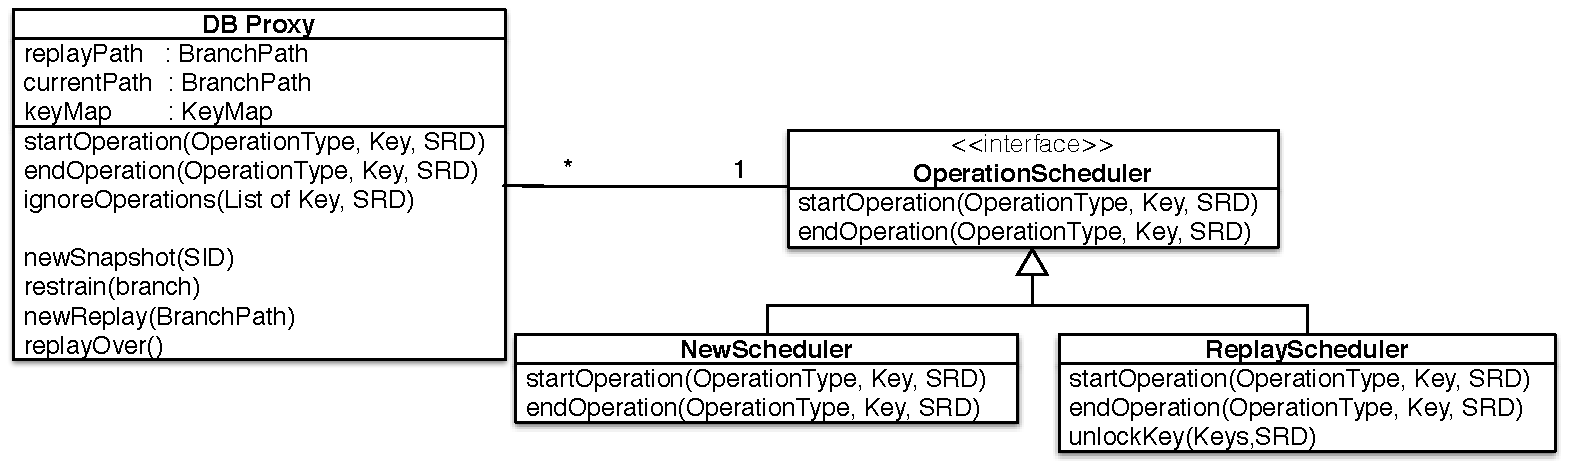
\includegraphics[width=\textwidth]{arch/scheduler_uml}
  \caption{UML of Database proxy and schedulers}
  \label{fig:scheduler_uml}
\end{figure}

%How to distinguish between new requests and replay requests? The replay flag can be removed
Each database proxy maintains two \emph{branch path}. A branch path of a certain branch is the sequence of non-tampered snapshots between the current snapshot and the root snapshot (Chapter \ref{sec:arch:runtime_recovery}). The first branch path, named \textit{current branch}, refers to the branch used by new incoming requests, while the second, named \textit{replay branch}, wraps the branch used by the requests being replayed.

Before each replay process, the Shuttle manager sends the branch path of the new replay branch, in which the requests will be replayed. At the end of replay process, the database nodes are also notified and the \textit{replay branch} becomes the \textit{current branch}. If the branch of the request is the \textit{replay branch}, then it is being replayed. Otherwise, it is a new request.\\


%New operations
First, we consider operations of new incoming requests. Shuttle tracks operations of new requests and allows a single write or multiple read operations per key. To do so, the Shuttle interceptor invokes the \emph{newScheduler}, which invokes the \emph{keyMap} (Figure \ref{fig:sequence_normal}). The \emph{keyMap}, which is the main data structure of database proxy, is a concurrent hash table that binds each  key to its Shuttle metadata, named \emph{keyMapEntry}. To improve Shuttle's performance, the \emph{keyMap} is internally partitioned to permit concurrent reads and updates.

\begin{figure}
  \centering
  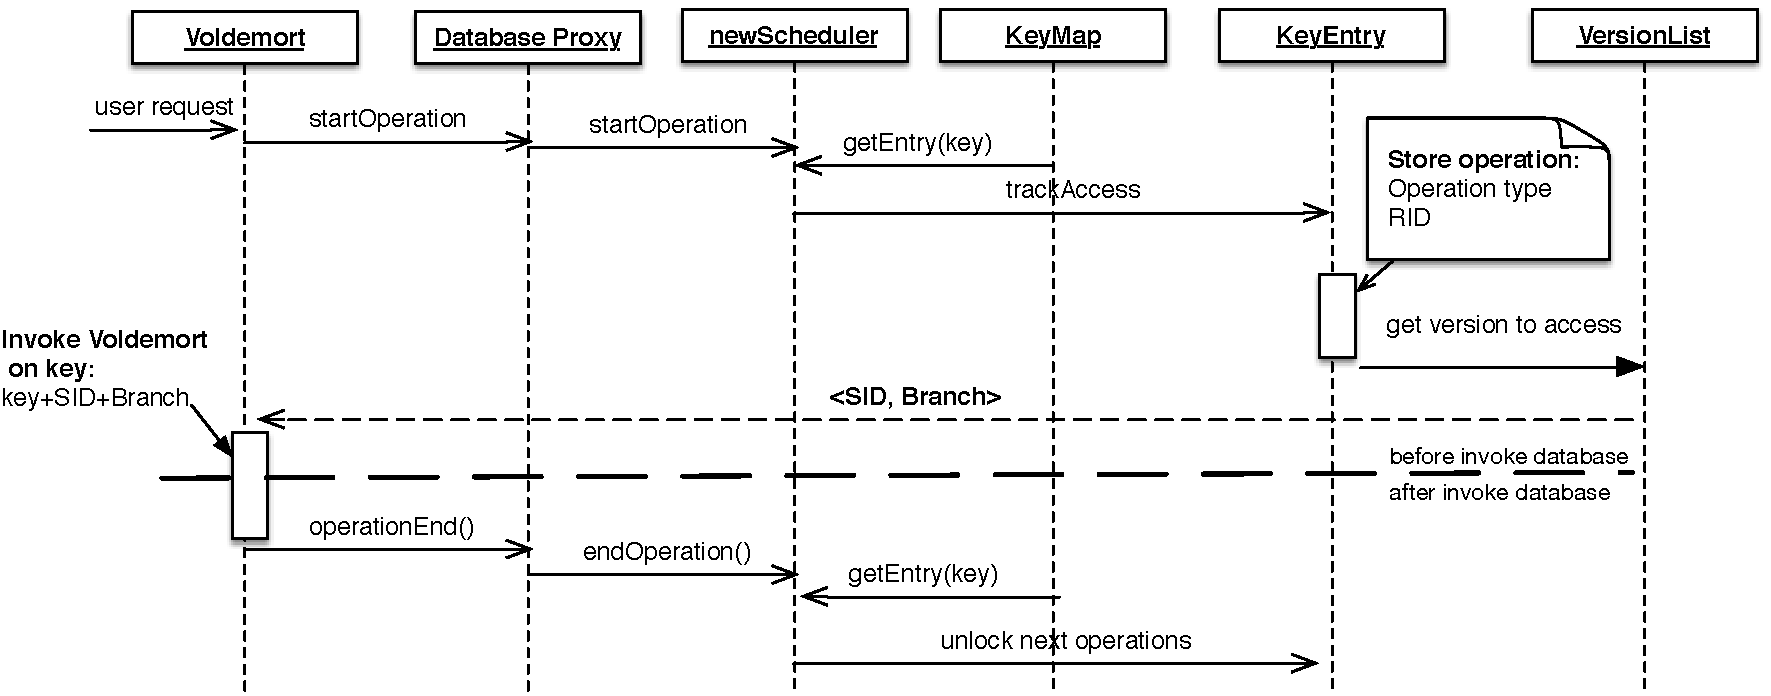
\includegraphics[width=\textwidth]{arch/operation_database}
  \caption{Sequence of invocations between the main data structures of database proxy }
  \label{fig:sequence_normal}
\end{figure}


Each \emph{keyMapEntry} object wraps the Shuttle metadata for one key/data-item: \emph{version list}, \emph{operation list} and \emph{read-write lock} (Figure \ref{fig:keymap}). The \emph{version list} contains the list of versions: snapshot in which the entry has been written. A data item may not be written in every snapshot (Section \ref{sec:arch:runtime_recovery}). 

\begin{figure}
  \centering
  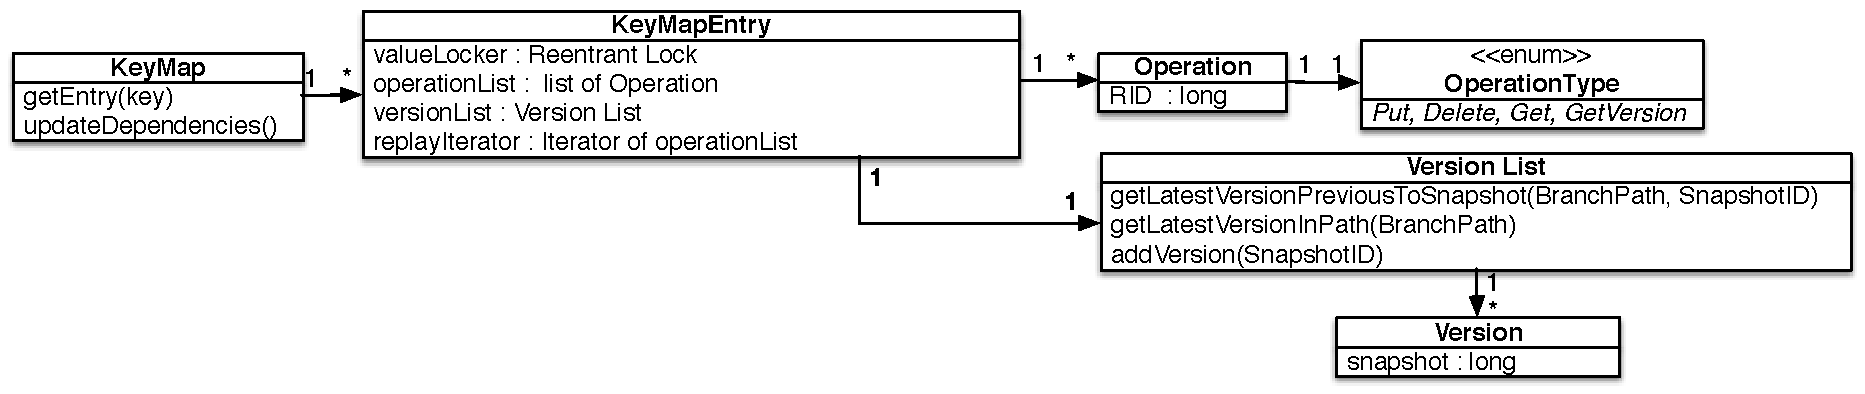
\includegraphics[width=\textwidth]{arch/keymap}
  \caption{KeyMap UML: the entities used to to track operations and versions of each key.}
  \label{fig:keymap}
\end{figure}


The \emph{operation list} contains the sequence of operations of a certain key (data item). Each operation has an operationType (put, get, delete, get version) and the \ac{RID} of the retrieved requests. The \emph{read-write lock} lock serializes the operation that access the key value allowing concurrent reads or a single write at each time. This pessimistic concurrency control method may decrease the system performance comparing, for instance, with a multi-version concurrency control. An alternative implementation can write the \ac{RID} among the value in the store and track only the read accesses, parsing the accessed \ac{RID}. The client library may parse the value to get the \ac{RID} but the write order is relevant. For sake of simplicity, we used a pessimistic concurrency control with a reentrant mutual exclusion lock.\\

%Read/Write lock, add operation and get the correct version
When \emph{newScheduler} is invoked by an operation from a new incoming request, it gets the \emph{keyMapEntry} of the key and attempts to gain the access to its \emph{read-write lock} (Algorithm \ref{code:snapshotAlgorithm}). Then, it adds the operation to the \emph{operation list}. At last, Shuttle gets the correct version to access based on the \emph{branch path} and the \emph{list of versions} of the key (Section \ref{sec:arch:runtime_recovery}). 

If the request \ac{RID} is smaller than the current \ac{SID} (line \ref{line:snapshot:1}), then the request does not belong to the current snapshot and shall access the latest, but previous to the snapshot instant, version of the value that is in the  \textit{current branch path}. Otherwise, the request belongs to the current snapshot. Read operations access the latest version (line \ref{line:snapshot:2}) in the  \textit{current branch path}. A write request may create a new version if the version has yet not been written in the current snapshot (\ac{RID} is bigger than the \ac{SID} of the latest version) (line \ref{line:snapshot:3}). Versions are created with the current \ac{SID}. The key accessed by the request is the concatenation of the original key with the version returned by the Algorithm \ref{code:snapshotAlgorithm}. After the access, the \emph{read-write lock} is unlocked and the next operations proceed.


\begin{algorithm}
\DontPrintSemicolon\SetKwProg{fn}{Function}{}{}
\SetKwFunction{TrackAccess}{trackAccess}\SetKwFunction{AddOperation}{operationList.add}
\SetKwFunction{WriteLock}{lock.writeLock}\SetKwFunction{ReadLock}{lock.readLock}
\SetKwFunction{AddVersion}{versionList.add}

	% \KwData{$map$ is a static hash table}
	% \KwIn{HTTP user request and \ac{HTTP} response}
	\BlankLine
	\fn{\TrackAccess{operation type, srd, branch path}}{
		\eIf{type is put or delete}{
			\WriteLock{}\;
		}{
			\ReadLock{}\;
		}
		\BlankLine
		\AddOperation{new Operation(type, srd.rid)}\;
		\BlankLine
		\eIf{srd.rid < branch path.sid}{  \label{line:snapshot:1}
			\tcp{Access only the versions of previous snapshots}
			\Return latest version in $(version list \cap branch path : version < srd.rid)$\;
		}{
			\tcp{Access the latest version}
			\Letv{latest}{get latest version in $(version list \cap branch path)$}\;
			\If{type is get}{
				\Return	 $latest$\; \label{line:snapshot:2}
			}
			\tcp{New version is created if the request belongs to a newer snapshot}
			\If{branch path.sid > latest.sid}{ \label{line:snapshot:3}
				\Letv{version}{new Version(branch path.sid)}\; 
				\AddVersion{version}\;
				\Return{version}\;
			}
		}
	}{}
	 \caption{Method to track a new request, get the version to access and perform snapshot}
	\label{code:snapshotAlgorithm}
\end{algorithm}

Since the \emph{version list} keeps a pointer to the latest version and the pointer is updated if wrong, the average complexity of the Algorithm \ref{code:snapshotAlgorithm} is \O{1}: get the latest version and check if it belongs to the branch path, which is a HashSet. If the branch path size becomes a considerable storage overhead, the branch paths and version lists can be implemented as a bitmaps.\\

\begin{figure}
  \centering
  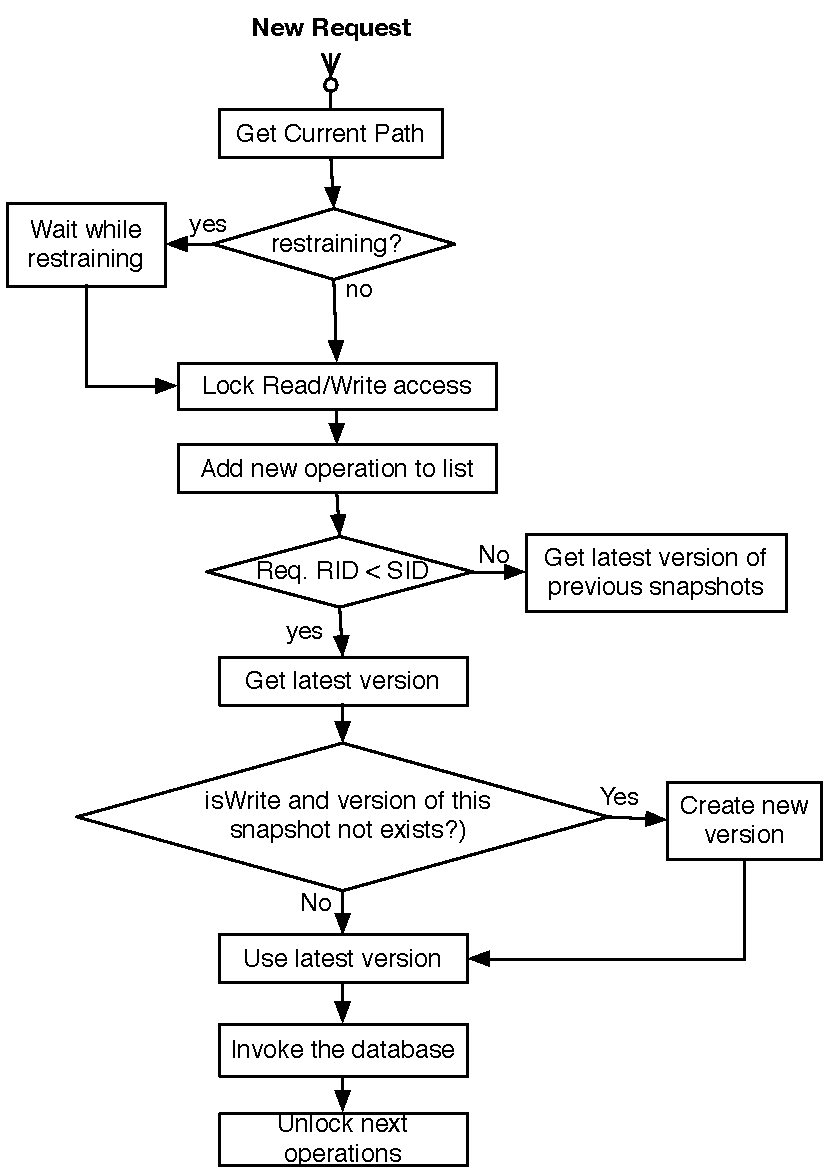
\includegraphics[width=80mm]{arch/database_proxy_logics}
  \caption{Diagram of processing a new database request}
  \label{fig:impl:database:process_new}
\end{figure}
	
%collect dependencies
Shuttle collects the dependencies between requests transversing the operation list of every \emph{KeyMapEntry} in the \emph{KeyMap}. Each \emph{KeyMapEntry} keeps a pointer to the latest collected dependency in the operation list, so only new operations are transversed.

In order to determine the dependencies between requests, Shuttle firstly lookup for the write operation previous to the latest collected operation (Algorithm \ref{code:dependency_collection}). Then, it iterates the operations following to the latest collected operation. If an operation of request $A$ reads a data item written by an operation of request $B$, then $A$ depends on $B$. Dependencies are logged on a hash table that associates the operation \ac{RID} with the \ac{RID}s which it depends on. Every database node sends its $dependenciesTable$s to the manager periodically. 

 
\begin{algorithm}[H]
\DontPrintSemicolon\SetKwProg{fn}{Function}{}{}
\SetKwFunction{Add}{dependencies.add}
	\SetKw{KwInit}{Initialization:}\KwInit{\Letv{dependencies}{new hash table<Long,Long>}}\;
	\BlankLine
	\ForEach{$entry$ in $keyMap$}{ 
		\Letv{lastWrite}{\ac{RID} of the latest write operation previous to the earlier operation to collect}\;
		\ForEach{operation \textbf{in} entry.operationList}{
			\eIf{operation.type == READ}{
				\Add{operation.rid, lastWrite}\;
			}{
				\Letv{lastWrite}{operation.rid}\;
			}
		}
		\Letv{entry.lastCollected}{latest operation in $entry.operationList$}\;
	}
	\BlankLine
	send $dependenciesMap$ to manager\;

 \caption{Dependency collection}
\label{code:dependency_collection}
\end{algorithm}


%Scalability
\acs{NoSQL} databases are designed for distributed environments. The proposed dependency tracking and snapshot mechanisms are horizontally scalable: each database node remains independent and each data item is independent from the others. The only locks shared by data items are the KeyMap partition lock and the KeyMapEntry lock. Adding more partitions, can improve the overall performance. Each node is responsible for logging local dependencies and communicates to a central entity (Manager) to update the  dependency graph. 


\subsection{Manager}\label{sec:impl:normal:manager}
%summary
The main duties of manager are: retrieve dependencies between database operations and generate the dependency graph; coordinate database nodes to create new database snapshots; coordinate the recovery process. 

%When and how retrieves
In order to generate the dependency graph, dependencies are pushed to the manager by the database nodes. The dependency graph is updated during the normal execution. An alternative approach could pull the dependencies from each database node during the recovery phase and generate the graph during the recovery period.

%Definition
The dependency graph is a set of vertexes, each one representing a request, and a collection of edges that each connect a pair of vertexes. Each edge specifies an one-way dependency between two requests. Therefore, the dependency graph is a directed graph. The dependency graph is also \emph{not connected}, i.e., it consists of a set of connected subgraphs. Each vertex is uniquely identified by its key, the \ac{RID} of the request that it represents. 


The dependency graph has four main operations: insert new dependencies, get requests sorted by start instant, get requests dependent from a certain request, get requests from which a certain request depends on.

The first operation inserts new vertexes (requests) and adds edges between the new vertexes and all vertexes from which new vertexes depends on. The second visits every vertex by the order of their key (start instant). The two latest operations visit all vertexes reachable from a certain vertex using the \emph{dependencies to} and the \emph{dependencies from} directions, respectively. Even the dependency graph is, conceptually, a directed graph, the two latest operations are easier to implement on \emph{undirected graphs}.

Two of the main representations of graphs in memory are: adjacent matrix and adjacent list. On a dependency graph, each insert operation requires to create several edges, one per dependency. An edge can be inserted on an adjacency matrix with complexity \O{1}. However, we consider the dependency graph to be a \emph{sparse graph} because each request is expected to be dependent from a small part of all requests. Therefore, the adjacent list representation is expected to be more space efficient than the matrix.

The three main implementations of a adjacent list graph are: an indexed array, object oriented (nodes with pointers) and a hash table. The vertex keys are expected to be a sparse numeric sequence with irregular number of edges. Therefore an indexed array implementation would not be space efficient. Insert operations in object oriented graphs requires searching for objects to create new edges. However, a graph search algorithm, for instance breadth-first search (BFS), has a time complexity of \O{|Vertix|+|Edges|} in the worst case.
Hash table implementations use a hash table to associate each vertex in a graph with an array of adjacent vertexes. To clarify, each hash table object represents a vertex. The object has list of keys that represents the edges. \\

We implemented the dependency graph as a hash table. Doing so, insert operations have \O{1} complexity. Operations to obtain the first level of dependencies of a certain requests has also have \O{1} complexity. Even so, we also take in consideration that the performance of these operations is influenced by constant factors and by the hashing function and data distribution.

The hash table keys are the \ac{RID}, which is also the start timestamp of the request. The object associated with each key wraps: the end timestamp; the list of requests from which the request depends on (executed before); the list of requests dependent from the request (to execute after) (Figure \ref{fig:impl:manager:graph}). For sake of simplicity, the graph is kept in the memory of the manager. A production mode implementation, in which the memory limit can become a bottleneck, shall implement the dependency graph in a \ac{DHT} or a key-value \acs{NoSQL} store.


\begin{figure}
  \centering
  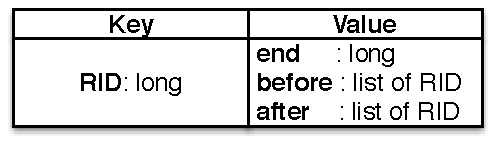
\includegraphics[width=50mm]{arch/managerGraph}
  \caption{Entry of the dependency graph HashMap}
  \label{fig:impl:manager:graph}
\end{figure}


%how it stores the dependencies
The manager updates the dependency graph when a new table of dependencies is retrieved from a database node (Algorithm \ref{code:add_dependency_graph}). The retrieved hash table associates each \ac{RID} with the \ac{RID} of the requests from which the request depends on. The algorithm creates an undirected graph, which can be considered as two directed graphs: the first representing the dependencies from; the seconds the dependencies two. In other words, the graphs are symmetric: one graph can be generated inverting the directions of the edges of the other graph.\\

 \begin{algorithm}[H]
 \DontPrintSemicolon\SetKwProg{fn}{Function}{}{}
 \SetKwFunction{Add}{entry.addBefore}\SetKwFunction{AddAfter}{entry.addAfter}
 	\KwIn{\Letv{dependencies}{HashTable<RID, list of RID>}}\;
 	\BlankLine
 	\ForEach{$\{rid, dependencyList\}$ in $dependencies$}{
 		\Letv{entry}{get or create a GraphEntry in dependency graph for $rid$}\;
 		\Add{$dependencyList$}\;
 		\BlankLine
 		\ForEach{$dependentRID$ in $dependencyList$}{
	 		\Letv{entry}{get or create a GraphEntry in dependency graph for $dependentRID$}\;
	 		\AddAfter{rid}\;
 		}
 	}
 	\caption{Add dependency to dependency graph}
	\label{code:add_dependency_graph}
\end{algorithm}

%Branching
The manager maintains the \textit{BranchTree}. BranchTree is the implementation of the branching model introduced in Chapter \ref{sec:arch:runtime_recovery}. The BranchTree is implemented as a hash table that associates each branch and its snapshots. The tree model allows tenants to create new branches or snapshots.

In order to create a snapshot, tenants define a future instant in time, $t$, when the snapshot will occur. The manager forwards the value of $t$, named \ac{SID}, to every database instance. Each database node adds a new snapshot with the retrieved \ac{SID} in the \emph{current branch path}. The manager insert the \ac{SID} in the entry of the current branch in the \emph{BranchTree}.

In order to create a new branch and start a new replay process, tenants shall specify a base snapshot. The branching algorithm finds the branch of the selected snapshot and copies the snapshots in the list, which are equal or previous to the selected snapshot, to create a new entry in the BranchTree for the new branch. Then, the algorithm creates a snapshot in the new branch. In other words, the new branch path is the concatenation of the new snapshot, in which the replay will be written, and the sequence of snapshots of the branch of the selected snapshots that are equal or previous to it. The new branch path is send to the database proxy of all database nodes.\\


%Communication
Shuttle's manager prototype retrieves tenant's commands via command line. Each module of Shuttle, including the manager, has a TCP server that retrieves requests from other modules. Requests are formatted using Google's Protocol Buffer \cite{protobuffers}. Messages exchanged between the manager and the remaining modules are in Appendix \ref{appendix:shuttle_api}. 



\section{Recovery}\label{sec:impl:recovery}
%overview
In this section, we introduce the implementation of the recovery process in Shuttle.\\

The recovery process begins when the tenant selects a non-tampered snapshot. The manager creates a new branch and sends its \emph{branch path} to all database proxies. The proxies set the new branch path as \emph{replay branch} (Chapter \ref{sec:impl:normal:database}). After, the manager generates the sequence of requests to replay, named \emph{execution list}. The replay instances are launched and retrieve this list (Figure \ref{fig:messaging_replay}). Then, the replay instances are notified to start replaying the requests. After replaying all the requests, each replay instance notifies the manager. The manager sets the proxy state to \emph{restraining mode} and commands the replay instances to replay the incoming requests retrieved during the recovery period. After replaying the remaining requests, the database nodes are notified to disable the restrain and \emph{replay branch} becomes the \emph{current branch}. At end, the proxy \emph{restraining mode} is disabled and the following new requests are done in the new branch.

\begin{figure}
  \centering
  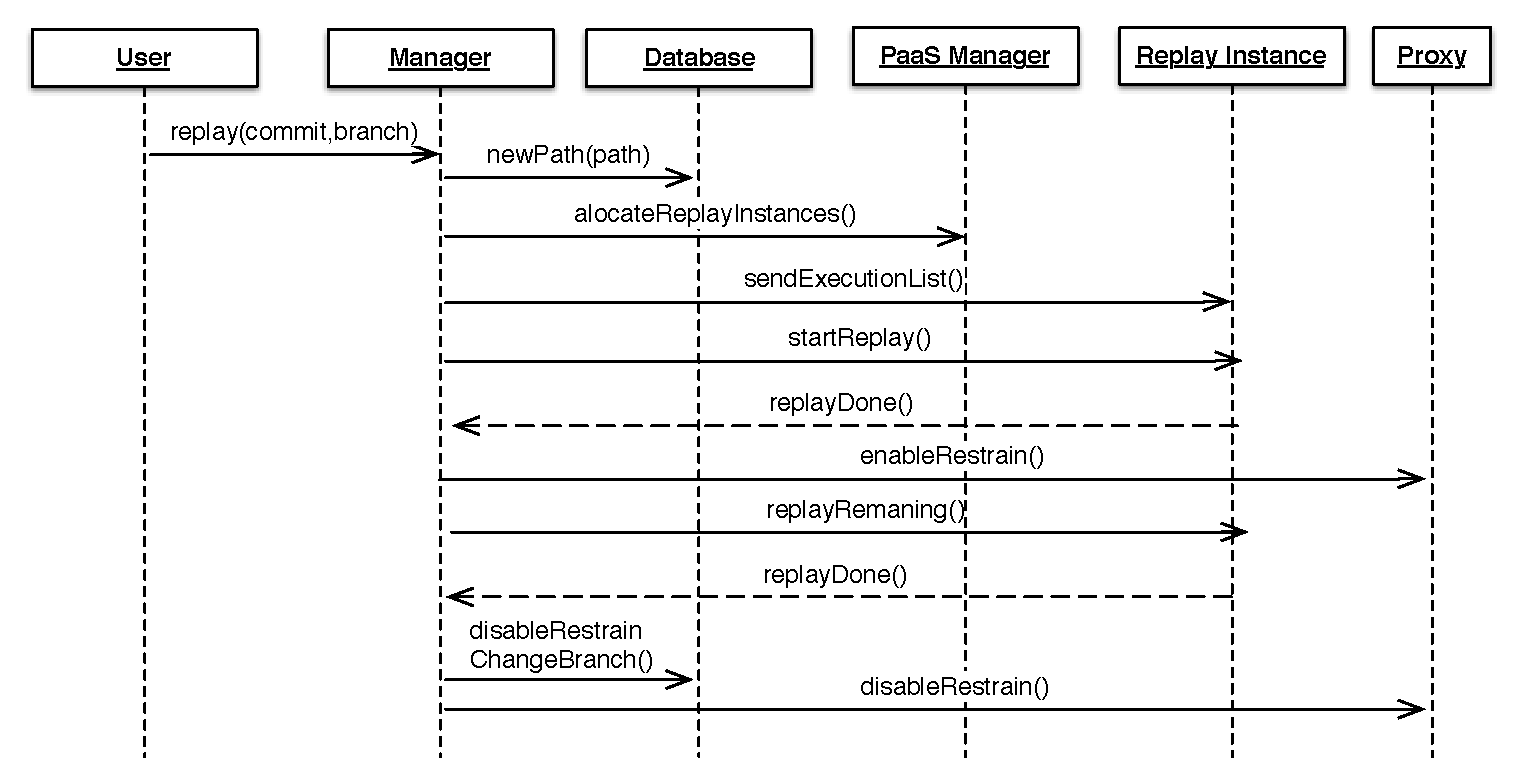
\includegraphics[width=140mm]{images/message_replay}
  \caption{Message sequence during replay phase}
  \label{fig:messaging_replay}
\end{figure}


\subsection{Manager}\label{sec:impl:recovery:manager}
Tenants start the recovery process by selecting a snapshot that does not contain the result of any malicious action. Shuttle creates a new branch and sends its \emph{branch path} every database proxy. After, the manager generates the request execution list, i.e., the sequence by the requests shall be replayed.

Shuttle can perform selective or full replay. It also can use clustering to re-execute different sequences of requests in parallel or not (Table \ref{tab:operation_types}).

%full-replay
Shuttle uses the Algorithm \ref{code:start_end_full_replay} to generate a request execution list for full-replay. The algorithm implements the start-end request ordering approach presented in Section \ref{sec:arch:dependencies}. Since the graph is implemented as a hash table (Section \ref{sec:impl:normal:manager}), the keys are not ordered. At recovery time, the keys are ordered and the graph is iterated in order. The complexity of this operation is \O{n \log{} n}. A request must be executed concurrently with a previous request if it began before a previous request ends. Otherwise, the request was not executed concurrently with any of the previous requests.

\begin{algorithm}[H]
\DontPrintSemicolon\SetKwProg{fn}{Function}{}{}
\SetKwFunction{Max}{max}
	  \KwIn{$graph$: dependency graph (Hash Table)}
	  \KwIn{$snapshot$: non-tampered \ac{SID} selected by the tenant }
	  \KwOut{$executionList$: sorted list of \ac{RID} to replay}
	  \BlankLine
	  Sort $graph$ keys\;
	  \BlankLine
	  \Letv{latestExecuting}{-1}\tcp*{the biggest end timestamp being executed}
	  \ForEach{$request$ in $graph$}{
	      \eIf{$request.start => latestExecuting$}{
	      	  
	          add $separator$ to $executionList$ \tcc{none of following requests were executed concurrently with previous}
	      }{
	          add $request$ to $executionList$\;
	      }
	      \Letv{latestExecuting}{\Max{latestExecuting,request.end}}\;
	  }
	\caption{Start-end ordering algorithm}
	\label{code:start_end_full_replay}
\end{algorithm}


%clustering
The clustering mechanism identifies the connected subgraphs of the dependency graph. The algorithm traverses the vertex marking all adjacent nodes that are reachable from a node. The set of nodes reachable from a node defines a cluster. Then, we choose a non-marked node and repeat the procedure.\\

%selective-replay
When the tenants provide a set of malicious actions, $A_{intrusion}$, Shuttle performs selective replay instead of replaying every request. Selective replay uses the dependencies between requests to expand a provided set of malicious requests, $A_{intrusion}$,  to get which requests are needed to be replayed. The set of malicious requests is expanded adding all requests dependent from the initial malicious request set. The traversed nodes are the tainted requests, $A_{tainted}$. Then, the set $A_{tainted}$ is expanded transversing the nodes of the set on the opposite direction: visit requests from which the traversed node depends on and that are posterior to the selected snapshot (Figure \ref{fig:selectiveGraph}). 


The list of data items read by the requests in $A_{replay}$ is obtained querying the Shuttle storage. The storage contains the keys accessed per request, which was logged by the application servers (Section \ref{sec:impl:normal:compute}). The snapshot versions of these items is loaded and the requests in $A_{replay}$ are replayed. The modified data items are merged with the current database values without copying data values. To do so, the \emph{branch path} of a selective replay branch contains the current \emph{branch path}. This mechanism avoids tainting the modified data items and copying them into the current database state. This mechanism does not support runtime recovery but the recovery period is considerably smaller than using full-replay.

%\item \textit{If a replayed request operation a different entry, then the requests which access the entry are also replayed.}
%During the replay phase, requests may access different data items than the ones during the first execution. If the value of the data item is not-updated because non of the tainted requests accessed the entry before, then, every request that access the entry is also tainted and replayed before the current access proceed.
%After each replayed request, the performed database operations are compared with the original set of operations. For each key of the operations performed originally but not in the replay, are unlocked. For each key of the operations performed on replay but not originally, the following operations are also replayed. 


\subsection{Replay Instances}\label{sec:impl:recovery:replay}
%How they can work?
The Shuttle manager requires the \ac{PaaS} controller to launch a set of \textit{replay instances}. If the \ac{PaaS} system does not support auto-scaling, the manager requests the \ac{PaaS} controller to add new database and application instances to attend the flow of replayed requests. Otherwise, the auto-scaling mechanism will detect the overload of the application and database instances and trigger the creation of new instances. In the first case, the number of application instances is constant during the replay phase, so the instances send the requests directly to the application instance instances, avoiding the overhead of the load-balancer. In the second case, the requests are sent to the load-balancer that distributes the requests through the instances. In the current implementation, requests are sent to the load-balancer because AppScale supports auto-scalling and the number of instances during the replay phase is unknown.\\

%How they they are implemented to work
Each replay instance retrieves a set of lists of \ac{RID} to execute and the branch in which they shall be executed. Replay instances have a main thread to schedule the execution and a thread pool to execute requests asynchronously. Each thread fetches the \acs{HTTP} requests from the \emph{Shuttle storage}, modifies their header setting the \ac{SRD} field \emph{branch} and sends them to the load-balancer. Each response is compared against the response during first execution. An alternative approach can compute the hash of responses in background and compare their values.

If a request has been removed, for instance if it is a malicious request, the replay instance fetches the keys accessed by the malicious request during its first execution and invokes the database proxy to unlock the execution.\\ %An alternative approach using a distributed lock per data item does not require to store the accessed keys but requires to store the replayed requests and share a lock, which can be a bottleneck. 

The prior evaluation, on serial-replay schema, showed fetching each request before sending is a considerable overhead. We duplicated the throughput and reduced the Shuttle storage usage by using a thread in background to fetch batches of requests from the Shuttle storage. The fetching thread and the execution threads communicate through a in-memory message queue.

%Flow control
The start-end algorithm (Algorithm \ref{code:start_end_full_replay}) groups the requests that shall be executed concurrently. The separator marks the end of a group of concurrent request. When a separator is reached in the request list, the execution thread waits until all responses are retrieved. Even so, the number of concurrent requests within a group can overload the servers and database instances. In addition, since application server and replay instances are supported by thread pools, the system reaches a \emph{deadlock} if all threads of one of the thread pools are blocked waiting for further requests. Taking that in consideration, all components in Shuttle shall be asynchronous and message-driven.

%Goal:
%1 - O client envia o pedido e segue o processamento do próximo
%2 - A base de dados tenta processá-lo. Se não conseguir, cria um future e prossegue.
%3 - Quem acaba e ia acordar os bloqueados, agora invoca o future para que este seja processado
%4 - A resposta é return e o client detecta o evento de nova resposta, invoka a callback e prossegue com o pedido.

%O DBProxy deveria ser semelhante a um serviço de queue e workers para que os pedidos possam ser devolvidos à queue e os workers possam continuar a processar outros pedidos. Alterantiva: usar o modelo de queue de mensagens: guardo os pedidos que tenho para processar se não derem para ser processados agora e depois, verifico se já os posso processar. volto a processá-los depois.

%A alternativa tem de ser um client baseado em callbacks. Envia o pedido, continua para outros pedidos e quando vier a resposta, associa-a ao pedido e prosseegue... problema: isto não existe em voldemort. o cassandra faz mas o voldemort não.


As requests are replayed asynchronous, the replay instances must use an end-to-end flow control protocol to avoid the sender send requests too fast for the application servers to receive and process. We implemented a simple flow control protocol, which does not have to lead with message ordering and retransmission because the underlying \ac{TCP} protocol handles transmission failures. We established two thresholds for the number of pendent responses that define 3 deltas on the request rates. Consequently, the request throughput of each replay instance is dynamic to avoid the servers overload. One of main challenges to evaluate the Shuttle's prototype is to tune the threshold parameters. Future implementations shall access the \ac{PaaS} controller in order to watch the instances' metrics and do flow control based on it.\\


\subsection{Database}\label{sec:impl:recovery:database}
%how it does replay?
In Section \ref{sec:impl:normal:database}, we introduced the \emph{newScheduler} of the Shuttle's database proxy. Schedulers intercept requests and define their execution order. The \emph{newScheduler} defines the order and logs the new operations. In this section, we introduce the \emph{replayScheduler}. This scheduler constrains the replayed operations, per data item, to an order consistent with the original execution of the application.

Database operations are processed by the replayScheduler if the \emph{branch} field of the operation \ac{SRD} is the same than \emph{replayBranch}. The replaySchedule gets the KeyMapEntry of the accessed key, which contains the list of operations logged during the execution phase. When the first operation, which is being replayed in current replay branch, accesses the data item, Shuttle creates an operation list iterator and associates it with the key.

The iterator of each operation list controls the replay process: it allows or blocks operations (Algorithm \ref{code:operation_iterator}). The iterator keeps a list of operations allowed, executing, waiting or to be ignored. The first allowed operation is the first operation after the snapshot selected by the tenant, i.e., the smallest \ac{RID} that matches the condition $\ac{RID} >= snapshot$ (line \ref{line:iterator:next}). 

When a new operation is retrieved, the iterator checks if there are operations executing or allowed to execute. If not, then the iterator transverses more operations of the list and adds them to the \emph{allowed list} (line \ref{line:iterator:fetch}). The algorithm fetches the following consecutive read operations or one write operation. Operations previous to the selected snapshot are not considered.

If an operation is not the following operation, i.e., operation $\notin$ allowed, then the operation is delayed and added to the \emph{waiting} list (line \ref{line:iterator:sleep}). Otherwise, the operation is allowed to proceed and is added to the \emph{executing} list.

After its execution, the operation is removed from the \emph{executing} list and blocked operations (in \emph{waiting list}) are unlocked to check if they can access. For sake of simplicity, the concurrency control is not included in the pseudo-code. \\

\begin{algorithm}[H]
\DontPrintSemicolon\SetKwProg{fn}{Function}{}{}
\SetKwFunction{Fetch}{fetchMoreAllowedOperations}\SetKwFunction{AllowedRemove}{allowed.remove}
\SetKwFunction{Executing}{executing.add}\SetKwFunction{WaitingAdd}{waiting.add}\SetKwFunction{WaitingRemove}{waiting.remove}
\SetKwFunction{AllowedAdd}{allowed.add}\SetKwFunction{Next}{iteratorNext}\SetKwFunction{ExecutingRemove}{executing.remove}
\SetKwFunction{StartReplay}{startReplayOperation}\SetKwFunction{EndReplay}{endReplayOperation}
 	\SetKwProg{KwInit}{Initialization}{:}{}
 	\KwInit{}{
 		\Indp
	 	\textit{all}: list of all operations\;
	 	\textit{allowed}: list of operations allowed to execute \;
	 	\textit{executing}: list of operations executing \;
	 	\textit{waiting}: list of operations waiting to execute \;
	 	\textit{ignoring}: set of operations to ignore \;
	 	\textit{nextOperation} $\leftarrow$ first operation after the snapshot\;
	}
 	\BlankLine
 	\BlankLine
 	\fn{\StartReplay{operation}}{
	 	\If{allowed is empty \emph{and} executing is empty} { \label{line:iterator:fetch}
	 	    \Fetch{}\;
	 	}
	 	\eIf{operation in allowed} {
	 		\tcp{move from allowed list to executing}	
	 		\AllowedRemove{operation}\;
	 	    \Executing{operation}\;
	 	}{
	 	    \WaitingAdd{operation}\;
	 	    thread sleep \tcp*{block operation} \label{line:iterator:sleep}
	 	    \WaitingRemove{operation}\;
	 	    \tcp{Attempt to execute}
	 	    \StartReplay{operation}
	 	}
	}
	\BlankLine
 	\BlankLine
 	\fn{\Fetch{}}{
 	 	\eIf{$nextOperation$ \textbf{is} write}{
 	 		\AllowedAdd{nextOperation}\;
 	 		\Letv{nextOperation}{\Next{nextOperation}} \;
 	 	}{
 	 		\tcc{add all read operations until next write}
 	 		\While{nextOperation \textbf{is not} write}{
 	 			\AllowedAdd{nextOperation}\;
 	 			\Letv{nextOperation}{\Next{nextOperation}} \;
 	 		}
 	 	}
 	}{}
 	\SetKwBlock{DoWhile}{do}{while}
 	\BlankLine
 	\BlankLine
 	\fn{\Next{operation}}{
 		\tcc{get next operation bigger than the base snapshot and not ignored}
 	 	\DoWhile{
 	 		\Letv{operation}{operation.next}\;
 	 	}\textbf{while} $operation.rid < SID$ \textit{or} $operation.rid \in ignoring$\; \label{line:iterator:next}
 	 	\Return{operation}
	}


 	\BlankLine
 	\fn{\EndReplay{op}}{
 		\ExecutingRemove{op}\;
 		\ForEach{operation \textbf{in} waiting}{
 			wake $operation$ thread\;
 		}
 	}{}
 \caption{Access iterator algorithm}
\label{code:operation_iterator}
\end{algorithm}


%unblock keys
The iterator ignores operations that belong to previous snapshot (line \ref{line:iterator:next}), i.e., $operation.rid < snapshot$, or to the \emph{ignoring} list. The \emph{ignoring} list contains the operations that will not be executed. If a request is malicious, the replay instances invoke the database \ac{API} method: $ignoreOperation(\ac{RID},keys)$ to ignore operations in all keys accessed by the request. In addition, when application servers retrieve requests and their replay flag is set, at the end of the request re-execution, the post-process interceptor of the database client library fetches the keys accessed by the requests during their first execution (Chapter \ref{sec:impl:normal:compute}). The process compares the keys accessed during the replay phase against the ones accessed during the first execution. The database client library invokes the method $ignoreOperation(\ac{RID},keys)$ to ignore the database operations that the request did not perform during the replay phase. This mechanism allows the blocked operations to proceed.

%If the request does not access all the keys than during its first execution, then the database client proxy invokes the same API. 
%\hl{justifica colocar o seguinte?:} An alternative approach could be: if a request locks, then it invokes a lock, which is shared between all database servers, informing which request should execute before it and waiting. When the request ends, the lock notifies the blocked processes. This approach does not require to store the accessed keys but requires to share a lock, which can be a bottleneck, and to store which requests have been replayed. 


%runtime recovery and change branch
Shuttle supports runtime recovery, i.e., the application remains online during the recovery process (Section \ref{sec:arch:runtime_recovery}). The field \emph{branch} contained in every request allows the database proxy to separate the operations of new incoming requests from the operations of requests being replayed. The first use the \emph{current branch} while the later use the \emph{replay branch}. As introduced above, the \emph{branch paths} and the scheduler algorithms define the versions which these operations read/write. This allows the new incoming requests to proceed during the recovery process.

At the end of the recovery process, the incoming requests must be switched to the application with fixed state, i.e., the requests should access the data items versions of the \emph{replay branch}. When all requests are replayed, the manager interact with the proxy to set the \ac{SRD} subfield \emph{restrain} in every following incoming request. The \emph{newScheduler} blocks the execution of new operations that have the \emph{restrain} flat set. Requests performed after the beginning of the replay process are replayed. After, the manager broadcasts a message to every database node to set the \emph{replay branch} as \emph{current branch} and ignore the restrain flag. The proxy is notified to stop setting the restrain flag. Consequently, the blocked requests and further new incoming requests are processed. This mechanism causes a delay on the request process in exchange for a simplicity and low communication overhead. 

%%%%%%%%%%%%%%%%%%%%%%%%%%%%%%%%%%%%%%%%%%%%%%%%%%%%%%%%%%%%%%%%%%%%%%%%%%%%%%%%%%%%%%%%%%%%%%%%%%%%%%%%%%%%%%%%%%%%%%%%%%%%%
\section{Application Example: Ask}\label{sec:impl:application}

We considered several application types to evaluate Shuttle. The selected application shall represent a generic web application, retrieve \ac{HTTP} requests and be deployable on AppScale. It should also fit the \acs{NoSQL} key-value store model and store its state in Shuttle version of Voldemort \cite{Kreps}. The selected application should imply dependencies between requests but unlike some web applications shall not imply external consistence issues. Accordingly, the application shall read only static data from other services, except the database.\\

We consider real-world applications such as office productivity, gaming, media content, data aggregation, wikis, diagramming and e-commerce applications (with shopping cart). For sake of simplicity, we developed \textit{Ask} instead of using real-world applications (Section \ref{sec:impl:application}). Even \textit{Ask} implementation is based on the real-world application StackExchange, its implementation is simpler than it. This allows to analyze the dependencies and reason about the results. We expect to evaluate the dependencies created by different types of application in future.

%explain the application
We developed a \ac{QA} web application, named \emph{Ask}, to evaluate Shuttle prototype. \emph{Ask} is based on Stack Exchange \cite{stackexchange} and Yahoo! Answers \cite{yahooAnswers}. The application data structure is as follows (Figure \ref{fig:DataStructure}). A question has a title, a known number of views by clients, a set of tags, which represent the themes of the question, and a set of answers. Each answer has a text and a number of user votes. Each user can only do a single vote per answer, incrementing or decrementing one unit the number of votes. Each answer has a set of comments.

 \begin{figure}
   \centering
   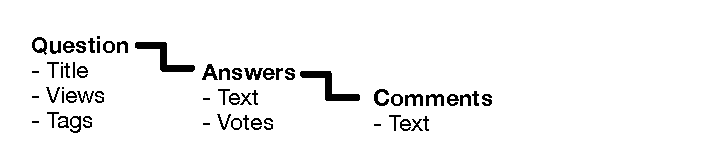
\includegraphics{images/questionStructure}
   \caption{Data structure}
   \label{fig:DataStructure}
 \end{figure}

The data is stored in four Voldemort stores (database schemas): questions, answers, comments and tags. For example, insert a new answer requires to add an entry to the \textit{answers store} and modify the entry of the corresponding question in \textit{questions store} to update the answer list. 

Independent user sessions would be trivial to replay in parallel. Therefore, the application semantics implies the following dependencies: a) questions are independent; b) a new answer depends on previous answers and votes to the same question; c) a new comment depends on the commented answer; d) a new vote depends on the voted answer (Table \ref{tab:dependencyTable}). In Chapter \ref{sec:eval:accuracy}, we compare the number of clusters considering or not dependencies between questions with the same tag.
\begin{table}
  \centering
   \begin{tabular}{l|l|l|l}
    ~             & \textbf{Read}   & \textbf{Write}   & \textbf{Depend on} 					 \\ \hline
    New Question  & (Tags)          & (Tags) Question  & (Tags)                                  \\ \hline
    New Answer    & Question        & Question, Answer & Previous answer to the same question     \\ \hline
    New Comment   & Answer          & Answer, Comment  & Commented answer                            \\ \hline
    New Vote      & Answer          & Answer, Vote     & Voted answer                               \\
    \end{tabular}
    \caption{Dependency list}
    \label{tab:dependencyTable}
\end{table}

Figure \ref{fig:dependencyGraph} represents an example of the application dependencies graph generated by Shuttle when two questions, two answers and one comment are created. Questions are independent, since they do not share a tag. Dashed entries represent read-only requests without consequent writes. A future work may consider to ignore these requests.

\begin{figure}
  \centering
  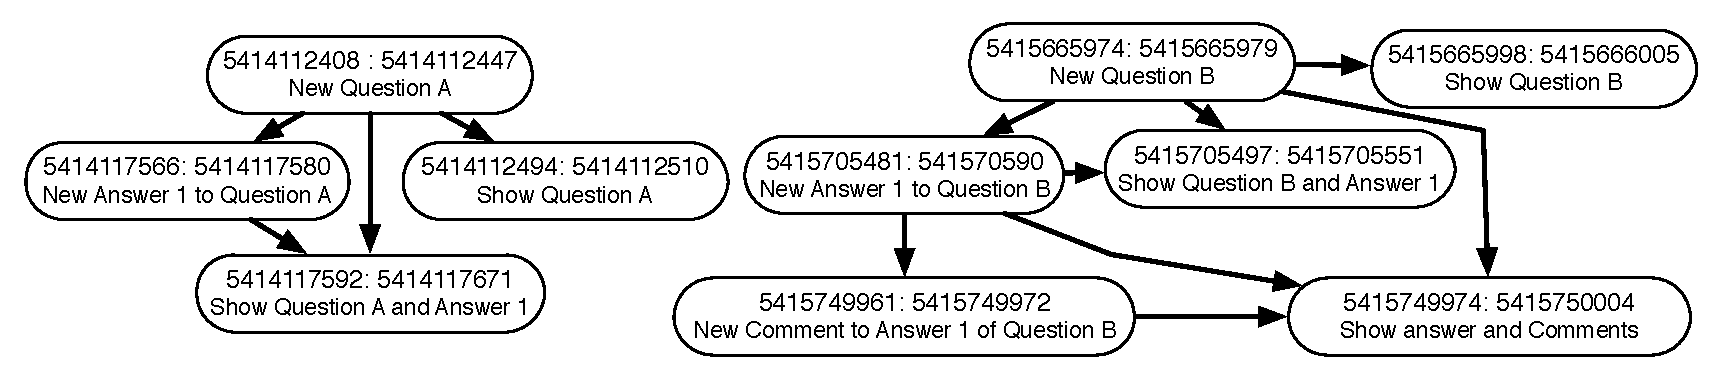
\includegraphics[width=150mm]{images/dependencyGraph}
  \caption{Example of a dependency graph generated by Shuttle}
  \label{fig:dependencyGraph}
\end{figure}

The application is implemented using Java Spring \cite{spring}, which is one of the most used Java enterprise web systems and it is compatible with most of the current \ac{PaaS} systems (Section \ref{sec:impl:adopted_technologies}). The implementation is independent of Shuttle. Shuttle does not require the application to be modified, except adding the Spring interceptor (Section \ref{sec:impl:normal:compute}). 


\section{Chapter Summary}\label{sec:impl:summary}
We presented the main implementation details of Shuttle prototype in Java. The total number of lines of code, except the unit tests, is summarized in Table \ref{tab:lines_of_code}.

The main development challenge is to implement 8 separate modules: TryOut master/slave, Proxy, Manager, Replay master/slave, database client interceptor, database proxy. In addition, the performance of each module is critical to demonstrate that this approach is valid. Therefore, each module is multi-thread and requires implementation of concurrency control. At least, the large data set implies issues with memory allocation.

\begin{table}[ht]
\centering
\begin{tabular}{lr}
\textbf{Components} 		& \textbf{Lines of code} \\ \hline
Proxy                      	& 1400    			\\   
Voldemort                  	& 1800    			\\
Manager                    	& 100     			\\    
Replay 			           	& 900     			\\    
Database Client Interceptor & 300     			\\     
TryOut                      & 3000    			\\    
Ask                         & 1700    			\\  \hline  
\textbf{Total}              & \textbf{11 000}  \\        
\end{tabular}
	\caption[Components of Shuttle prototype and an estimate of their complexity]
			{Components of Shuttle prototype and an estimate of their complexity, in terms of lines of code}
	\label{tab:lines_of_code}
\end{table}

